% Options for packages loaded elsewhere
\PassOptionsToPackage{unicode}{hyperref}
\PassOptionsToPackage{hyphens}{url}
%
\documentclass[
  ignorenonframetext,
]{beamer}
\usepackage{pgfpages}
\setbeamertemplate{caption}[numbered]
\setbeamertemplate{caption label separator}{: }
\setbeamercolor{caption name}{fg=normal text.fg}
\beamertemplatenavigationsymbolsempty
% Prevent slide breaks in the middle of a paragraph
\widowpenalties 1 10000
\raggedbottom
\setbeamertemplate{part page}{
  \centering
  \begin{beamercolorbox}[sep=16pt,center]{part title}
    \usebeamerfont{part title}\insertpart\par
  \end{beamercolorbox}
}
\setbeamertemplate{section page}{
  \centering
  \begin{beamercolorbox}[sep=12pt,center]{part title}
    \usebeamerfont{section title}\insertsection\par
  \end{beamercolorbox}
}
\setbeamertemplate{subsection page}{
  \centering
  \begin{beamercolorbox}[sep=8pt,center]{part title}
    \usebeamerfont{subsection title}\insertsubsection\par
  \end{beamercolorbox}
}
\AtBeginPart{
  \frame{\partpage}
}
\AtBeginSection{
  \ifbibliography
  \else
    \frame{\sectionpage}
  \fi
}
\AtBeginSubsection{
  \frame{\subsectionpage}
}
\usepackage{amsmath,amssymb}
\usepackage{lmodern}
\usepackage{ifxetex,ifluatex}
\ifnum 0\ifxetex 1\fi\ifluatex 1\fi=0 % if pdftex
  \usepackage[T1]{fontenc}
  \usepackage[utf8]{inputenc}
  \usepackage{textcomp} % provide euro and other symbols
\else % if luatex or xetex
  \usepackage{unicode-math}
  \defaultfontfeatures{Scale=MatchLowercase}
  \defaultfontfeatures[\rmfamily]{Ligatures=TeX,Scale=1}
\fi
\usetheme[]{Copenhagen}
\usecolortheme{dolphin}
\usefonttheme{structurebold}
% Use upquote if available, for straight quotes in verbatim environments
\IfFileExists{upquote.sty}{\usepackage{upquote}}{}
\IfFileExists{microtype.sty}{% use microtype if available
  \usepackage[]{microtype}
  \UseMicrotypeSet[protrusion]{basicmath} % disable protrusion for tt fonts
}{}
\makeatletter
\@ifundefined{KOMAClassName}{% if non-KOMA class
  \IfFileExists{parskip.sty}{%
    \usepackage{parskip}
  }{% else
    \setlength{\parindent}{0pt}
    \setlength{\parskip}{6pt plus 2pt minus 1pt}}
}{% if KOMA class
  \KOMAoptions{parskip=half}}
\makeatother
\usepackage{xcolor}
\IfFileExists{xurl.sty}{\usepackage{xurl}}{} % add URL line breaks if available
\IfFileExists{bookmark.sty}{\usepackage{bookmark}}{\usepackage{hyperref}}
\hypersetup{
  pdftitle={8- Hypothesis testing with qualitative variables},
  pdfauthor={Alex Sanchez, Miriam Mota, Ricardo Gonzalo and Santiago Perez-Hoyos},
  hidelinks,
  pdfcreator={LaTeX via pandoc}}
\urlstyle{same} % disable monospaced font for URLs
\newif\ifbibliography
\usepackage{color}
\usepackage{fancyvrb}
\newcommand{\VerbBar}{|}
\newcommand{\VERB}{\Verb[commandchars=\\\{\}]}
\DefineVerbatimEnvironment{Highlighting}{Verbatim}{commandchars=\\\{\}}
% Add ',fontsize=\small' for more characters per line
\usepackage{framed}
\definecolor{shadecolor}{RGB}{248,248,248}
\newenvironment{Shaded}{\begin{snugshade}}{\end{snugshade}}
\newcommand{\AlertTok}[1]{\textcolor[rgb]{0.94,0.16,0.16}{#1}}
\newcommand{\AnnotationTok}[1]{\textcolor[rgb]{0.56,0.35,0.01}{\textbf{\textit{#1}}}}
\newcommand{\AttributeTok}[1]{\textcolor[rgb]{0.77,0.63,0.00}{#1}}
\newcommand{\BaseNTok}[1]{\textcolor[rgb]{0.00,0.00,0.81}{#1}}
\newcommand{\BuiltInTok}[1]{#1}
\newcommand{\CharTok}[1]{\textcolor[rgb]{0.31,0.60,0.02}{#1}}
\newcommand{\CommentTok}[1]{\textcolor[rgb]{0.56,0.35,0.01}{\textit{#1}}}
\newcommand{\CommentVarTok}[1]{\textcolor[rgb]{0.56,0.35,0.01}{\textbf{\textit{#1}}}}
\newcommand{\ConstantTok}[1]{\textcolor[rgb]{0.00,0.00,0.00}{#1}}
\newcommand{\ControlFlowTok}[1]{\textcolor[rgb]{0.13,0.29,0.53}{\textbf{#1}}}
\newcommand{\DataTypeTok}[1]{\textcolor[rgb]{0.13,0.29,0.53}{#1}}
\newcommand{\DecValTok}[1]{\textcolor[rgb]{0.00,0.00,0.81}{#1}}
\newcommand{\DocumentationTok}[1]{\textcolor[rgb]{0.56,0.35,0.01}{\textbf{\textit{#1}}}}
\newcommand{\ErrorTok}[1]{\textcolor[rgb]{0.64,0.00,0.00}{\textbf{#1}}}
\newcommand{\ExtensionTok}[1]{#1}
\newcommand{\FloatTok}[1]{\textcolor[rgb]{0.00,0.00,0.81}{#1}}
\newcommand{\FunctionTok}[1]{\textcolor[rgb]{0.00,0.00,0.00}{#1}}
\newcommand{\ImportTok}[1]{#1}
\newcommand{\InformationTok}[1]{\textcolor[rgb]{0.56,0.35,0.01}{\textbf{\textit{#1}}}}
\newcommand{\KeywordTok}[1]{\textcolor[rgb]{0.13,0.29,0.53}{\textbf{#1}}}
\newcommand{\NormalTok}[1]{#1}
\newcommand{\OperatorTok}[1]{\textcolor[rgb]{0.81,0.36,0.00}{\textbf{#1}}}
\newcommand{\OtherTok}[1]{\textcolor[rgb]{0.56,0.35,0.01}{#1}}
\newcommand{\PreprocessorTok}[1]{\textcolor[rgb]{0.56,0.35,0.01}{\textit{#1}}}
\newcommand{\RegionMarkerTok}[1]{#1}
\newcommand{\SpecialCharTok}[1]{\textcolor[rgb]{0.00,0.00,0.00}{#1}}
\newcommand{\SpecialStringTok}[1]{\textcolor[rgb]{0.31,0.60,0.02}{#1}}
\newcommand{\StringTok}[1]{\textcolor[rgb]{0.31,0.60,0.02}{#1}}
\newcommand{\VariableTok}[1]{\textcolor[rgb]{0.00,0.00,0.00}{#1}}
\newcommand{\VerbatimStringTok}[1]{\textcolor[rgb]{0.31,0.60,0.02}{#1}}
\newcommand{\WarningTok}[1]{\textcolor[rgb]{0.56,0.35,0.01}{\textbf{\textit{#1}}}}
\usepackage{graphicx}
\makeatletter
\def\maxwidth{\ifdim\Gin@nat@width>\linewidth\linewidth\else\Gin@nat@width\fi}
\def\maxheight{\ifdim\Gin@nat@height>\textheight\textheight\else\Gin@nat@height\fi}
\makeatother
% Scale images if necessary, so that they will not overflow the page
% margins by default, and it is still possible to overwrite the defaults
% using explicit options in \includegraphics[width, height, ...]{}
\setkeys{Gin}{width=\maxwidth,height=\maxheight,keepaspectratio}
% Set default figure placement to htbp
\makeatletter
\def\fps@figure{htbp}
\makeatother
\setlength{\emergencystretch}{3em} % prevent overfull lines
\providecommand{\tightlist}{%
  \setlength{\itemsep}{0pt}\setlength{\parskip}{0pt}}
\setcounter{secnumdepth}{-\maxdimen} % remove section numbering
\ifluatex
  \usepackage{selnolig}  % disable illegal ligatures
\fi

\title{8- Hypothesis testing with qualitative variables}
\author{Alex Sanchez, Miriam Mota, Ricardo Gonzalo and\\
Santiago Perez-Hoyos}
\date{Statistics and Bioinformatics Unit. Vall d'Hebron Institut de
Recerca}

\begin{document}
\frame{\titlepage}

\begin{frame}
\begin{block}{Readme}
\protect\hypertarget{readme}{}
\begin{itemize}
\item
  License: Creative Commons Attribution-NonCommercial-ShareAlike 4.0
  International License
  \url{http://creativecommons.org/licenses/by-nc-sa/4.0/}
\item
  You are free to:

  \begin{itemize}
  \tightlist
  \item
    \textbf{Share} : copy and redistribute the material
  \item
    \textbf{Adapt} : rebuild and transform the material
  \end{itemize}
\item
  Under the following conditions:

  \begin{itemize}
  \tightlist
  \item
    \textbf{Attribution} : You must give appropriate credit, provide a
    link to the license, and indicate if changes were made.
  \item
    \textbf{NonCommercial} : You may not use this work for commercial
    purposes.
  \item
    \textbf{Share Alike} : If you remix, transform, or build upon this
    work, you must distribute your contributions under the same license
    to this one.
  \end{itemize}
\end{itemize}
\end{block}
\end{frame}

\begin{frame}[fragile]{Introduction}
\protect\hypertarget{introduction}{}
\begin{itemize}
\item
  Categorical variables represent facts that can be better described
  with \emph{labels} than with numbers.

  \begin{itemize}
  \tightlist
  \item
    Example: \texttt{Sex}, better choose from \{\texttt{Male} ,
    \texttt{Female}\} than from: \{1,2\}.
  \end{itemize}
\item
  Sometimes ordering of labels makes sense, although \emph{it is not
  reasonable to assign numbers to categories}:

  \begin{itemize}
  \item
    Example: \texttt{Tumor\ stage}: \{1,2,3,4\}, but \(1+2\neq 3\)!!!
  \item
    \texttt{Sex} is an example of a categorical variable in
    \texttt{nominal} scale
  \item
    \texttt{Stage} is an example of a categorical variable in
    \texttt{ordinal} scale
  \end{itemize}
\end{itemize}
\end{frame}

\begin{frame}[fragile]{Representing categorical variables in R}
\protect\hypertarget{representing-categorical-variables-in-r}{}
\begin{itemize}
\tightlist
\item
  Categorical variables are well represented with \emph{factors}
\end{itemize}

\begin{Shaded}
\begin{Highlighting}[]
\NormalTok{sex }\OtherTok{\textless{}{-}} \FunctionTok{factor}\NormalTok{(}\FunctionTok{c}\NormalTok{(}\StringTok{"Female"}\NormalTok{, }\StringTok{"Male"}\NormalTok{))}
\NormalTok{blood\_group }\OtherTok{\textless{}{-}} \FunctionTok{factor}\NormalTok{(}\FunctionTok{c}\NormalTok{(}\StringTok{"A"}\NormalTok{, }\StringTok{"B"}\NormalTok{, }\StringTok{"AB"}\NormalTok{, }\StringTok{"O"}\NormalTok{))}
\end{Highlighting}
\end{Shaded}

\begin{itemize}
\tightlist
\item
  Be careful with the names of factors, by default, \emph{levels}
  assigned in alphabetical order.
\end{itemize}

\begin{Shaded}
\begin{Highlighting}[]
\FunctionTok{levels}\NormalTok{(blood\_group)}
\end{Highlighting}
\end{Shaded}

\begin{verbatim}
## [1] "A"  "AB" "B"  "O"
\end{verbatim}

\begin{itemize}
\tightlist
\item
  To verify class of a variable
\end{itemize}

\begin{Shaded}
\begin{Highlighting}[]
\FunctionTok{class}\NormalTok{(sex)}
\end{Highlighting}
\end{Shaded}

\begin{verbatim}
## [1] "factor"
\end{verbatim}
\end{frame}

\begin{frame}[fragile]{Creating factors}
\protect\hypertarget{creating-factors}{}
\begin{itemize}
\item
  Factors can be created \ldots{}

  \begin{itemize}
  \item
    automatically, when reading a file or

    \begin{itemize}
    \tightlist
    \item
      Not all functions for reading data from file will create a
      factor!!!
    \item
      Usually levels will be defined from alphabetic order
    \end{itemize}
  \item
    using the \texttt{factor} or the \texttt{as.factor} commands.

    \begin{itemize}
    \tightlist
    \item
      more flexible
    \end{itemize}
  \end{itemize}
\end{itemize}
\end{frame}

\begin{frame}[fragile]{Create factors automatically}
\protect\hypertarget{create-factors-automatically}{}
\begin{itemize}
\item
  This is achieved by

  \begin{itemize}
  \item
    Using the \texttt{read.table} or \texttt{read.delim} functions for
    reading

    \begin{itemize}
    \tightlist
    \item
      Setting the ``character variables as.factors'' to TRUE
    \end{itemize}
  \end{itemize}
\item
  Example

  \begin{itemize}
  \tightlist
  \item
    Load the \texttt{diabetes} dataset using the
    \texttt{Import\ Dataset} feature of Rstudio

    \begin{itemize}
    \tightlist
    \item
      From text (base) (use the file \texttt{osteoporosis.csv})
    \item
      From text (readr) (use the file \texttt{osteoporosis.csv})
    \end{itemize}
  \item
    What is the class of the variable \texttt{menop}
  \end{itemize}
\end{itemize}
\end{frame}

\begin{frame}[fragile]{Create factors automatically}
\protect\hypertarget{create-factors-automatically-1}{}
\begin{Shaded}
\begin{Highlighting}[]
\NormalTok{osteo1 }\OtherTok{\textless{}{-}} \FunctionTok{read.csv}\NormalTok{(}\StringTok{"datasets/osteoporosis.csv"}\NormalTok{,}\AttributeTok{sep =} \StringTok{"}\SpecialCharTok{\textbackslash{}t}\StringTok{"}\NormalTok{,}
                   \AttributeTok{stringsAsFactors=}\ConstantTok{TRUE}\NormalTok{)}
\FunctionTok{class}\NormalTok{(osteo1}\SpecialCharTok{$}\NormalTok{menop)}
\FunctionTok{summary}\NormalTok{(osteo1}\SpecialCharTok{$}\NormalTok{menop)}
\FunctionTok{str}\NormalTok{(osteo1)}

\FunctionTok{library}\NormalTok{(readr)}
\NormalTok{osteo2 }\OtherTok{\textless{}{-}} \FunctionTok{read\_delim}\NormalTok{(}\StringTok{"datasets/osteoporosis.csv"}\NormalTok{, }\StringTok{"}\SpecialCharTok{\textbackslash{}t}\StringTok{"}\NormalTok{, }
                     \AttributeTok{escape\_double =} \ConstantTok{FALSE}\NormalTok{)}
\FunctionTok{class}\NormalTok{(osteo2}\SpecialCharTok{$}\NormalTok{menop)}
\NormalTok{osteo2}\SpecialCharTok{$}\NormalTok{menop }\OtherTok{\textless{}{-}} \FunctionTok{as.factor}\NormalTok{(osteo2}\SpecialCharTok{$}\NormalTok{menop)}
\FunctionTok{class}\NormalTok{(osteo2}\SpecialCharTok{$}\NormalTok{menop)}
\FunctionTok{summary}\NormalTok{(osteo2}\SpecialCharTok{$}\NormalTok{menop)}
\FunctionTok{str}\NormalTok{(osteo2)}
\end{Highlighting}
\end{Shaded}
\end{frame}

\begin{frame}[fragile]{Exercise 1}
\protect\hypertarget{exercise-1}{}
\begin{itemize}
\item
  Select \texttt{diabetes.xls} datasets
\item
  Read the dataset into R and check that the categorical variables you
  are interested (mort, tabac, ecg) in are converted into factors.
\item
  Confirm the conversion by summarizing the variables
\end{itemize}
\end{frame}

\begin{frame}{The analysis of categorical variables}
\protect\hypertarget{the-analysis-of-categorical-variables}{}
\begin{itemize}
\item
  The analysis of categorical data proceeds as usual:
\item
  Start exploring the data with the tables and graphics
\item
  Proceed to estimation and/or testing if \emph{appropriate}
\item
  Estimation

  \begin{itemize}
  \tightlist
  \item
    Proportions: Point estimates, confidence intervals
  \end{itemize}
\item
  Testing

  \begin{itemize}
  \tightlist
  \item
    One variable (tests with proportions)
  \item
    With two variables (chi-square and related)
  \end{itemize}
\end{itemize}
\end{frame}

\begin{frame}{Types of test with categorical variables}
\protect\hypertarget{types-of-test-with-categorical-variables}{}
\begin{itemize}
\item
  One variable (tests with proportions)

  \begin{itemize}
  \tightlist
  \item
    Does the proportion (\% affected) match a given value?
  \item
    Is the proportion (\% affected) the same in two populations?
  \end{itemize}
\item
  With two variables (chi-square and related)

  \begin{itemize}
  \tightlist
  \item
    Is there an association between two categorical variables?
  \item
    Is there a relationship between the values of a categorical variable
    before and after treatment?
  \end{itemize}
\end{itemize}
\end{frame}

\begin{frame}{Types of test with categorical variables}
\protect\hypertarget{types-of-test-with-categorical-variables-1}{}
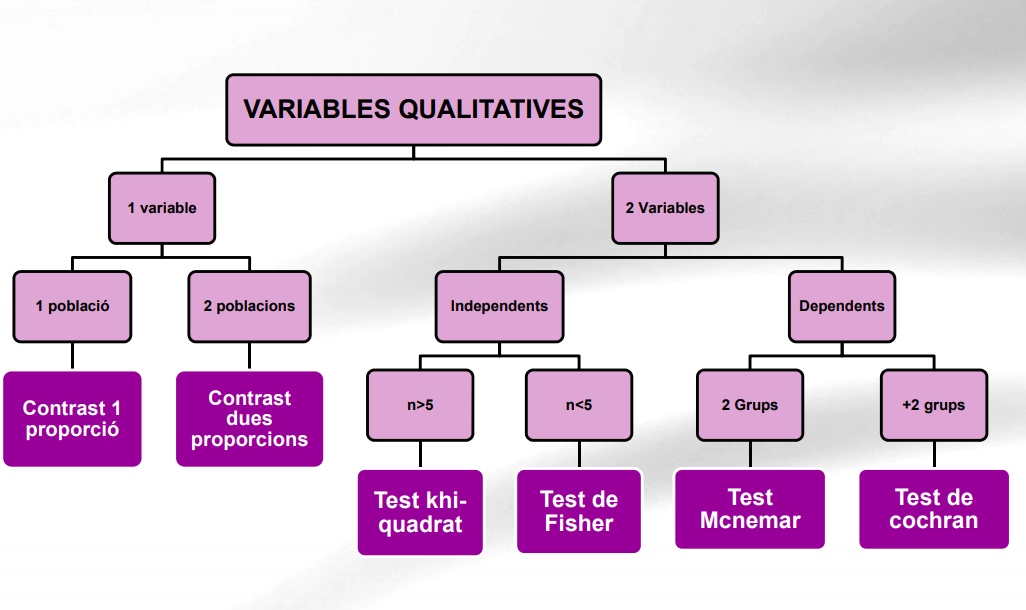
\includegraphics{images/arbrequali.PNG}
\end{frame}

\begin{frame}{Example}
\protect\hypertarget{example}{}
Consider the following study relating smoking and cancer.

\begin{figure}
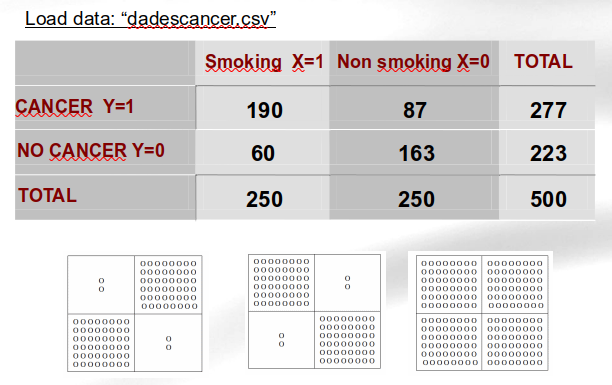
\includegraphics[width=0.8\linewidth]{images/cancerAndSmoking1png} \end{figure}

Our goal here would be to determine if there is an association between
smoking and cancer.
\end{frame}

\begin{frame}[fragile]{Crosstabulating a dataset}
\protect\hypertarget{crosstabulating-a-dataset}{}
\begin{itemize}
\item
  Data may come from a table (aggregated) or disagregated in a data
  file.
\item
  In this case we need to build the table applying ``cross-tabulation''
\end{itemize}

\begin{Shaded}
\begin{Highlighting}[]
\NormalTok{dadescancer }\OtherTok{\textless{}{-}} \FunctionTok{read.csv}\NormalTok{(}\StringTok{"datasets/dadescancer.csv"}\NormalTok{, }
                        \AttributeTok{stringsAsFactors =} \ConstantTok{TRUE}\NormalTok{)}
\end{Highlighting}
\end{Shaded}

\begin{Shaded}
\begin{Highlighting}[]
\CommentTok{\#attach(dadescancer)}
\NormalTok{mytable }\OtherTok{\textless{}{-}}\FunctionTok{table}\NormalTok{(dadescancer}\SpecialCharTok{$}\NormalTok{cancer, dadescancer}\SpecialCharTok{$}\NormalTok{fumar)}
\NormalTok{mytable}
\end{Highlighting}
\end{Shaded}

\begin{verbatim}
##            
##             Fuma No fuma
##   Cancer     190      87
##   No cancer   60     163
\end{verbatim}
\end{frame}

\begin{frame}[fragile]{Crosstabulation (2): Marginal tables}
\protect\hypertarget{crosstabulation-2-marginal-tables}{}
Marginal values are important to understand the structure of the data:

\begin{Shaded}
\begin{Highlighting}[]
\NormalTok{mytable}\OtherTok{\textless{}{-}} \FunctionTok{addmargins}\NormalTok{(mytable)}
\NormalTok{mytable}
\end{Highlighting}
\end{Shaded}

\begin{verbatim}
##            
##             Fuma No fuma Sum
##   Cancer     190      87 277
##   No cancer   60     163 223
##   Sum        250     250 500
\end{verbatim}
\end{frame}

\begin{frame}[fragile]{Crosstabulation (3): In percentages}
\protect\hypertarget{crosstabulation-3-in-percentages}{}
Showing tables as percentages is useful for comparisons

\begin{Shaded}
\begin{Highlighting}[]
\FunctionTok{prop.table}\NormalTok{(mytable) }\CommentTok{\# cell percentages}
\end{Highlighting}
\end{Shaded}

\begin{verbatim}
##            
##               Fuma No fuma    Sum
##   Cancer    0.0950  0.0435 0.1385
##   No cancer 0.0300  0.0815 0.1115
##   Sum       0.1250  0.1250 0.2500
\end{verbatim}

\begin{Shaded}
\begin{Highlighting}[]
\FunctionTok{prop.table}\NormalTok{(mytable, }\DecValTok{1}\NormalTok{) }\CommentTok{\# row percentages}
\end{Highlighting}
\end{Shaded}

\begin{verbatim}
##            
##                  Fuma   No fuma       Sum
##   Cancer    0.3429603 0.1570397 0.5000000
##   No cancer 0.1345291 0.3654709 0.5000000
##   Sum       0.2500000 0.2500000 0.5000000
\end{verbatim}

\begin{Shaded}
\begin{Highlighting}[]
\CommentTok{\# prop.table(mytable, 2) \# column percentages}
\end{Highlighting}
\end{Shaded}
\end{frame}

\begin{frame}{Exercise 2}
\protect\hypertarget{exercise-2}{}
\begin{itemize}
\tightlist
\item
  With the diabetes dataset repeat the crosstabulation done above using

  \begin{itemize}
  \tightlist
  \item
    Two categorical variables
  \item
    Variable ``mort'' and a newly created variable ``bmi30'' created by
    properly categorizing variable bmi.
  \end{itemize}
\end{itemize}
\end{frame}

\begin{frame}{One variable: Proportion tests}
\protect\hypertarget{one-variable-proportion-tests}{}
\begin{itemize}
\item
  According to medical literature, in the period 1950-1980, the
  proportion of obese individuals (defined as: BMI \(\geq 30\)) was 15\%
  in the population of men over 55 years old.
\item
  A random sample obtained from the same population between 2000 and
  2003 showed that, over a total of 723 men older than 55, 142 were
  obese.
\item
  With a significance level of 5\%, can we say that the population of
  men older than 55 in 2000-2003 had the same proportion of obese cases
  than that population had in 50'-80'?
\end{itemize}
\end{frame}

\begin{frame}[fragile]{Proportion tests with R}
\protect\hypertarget{proportion-tests-with-r}{}
Alternative ``NOT EQUAL''. This is set by default.

\begin{Shaded}
\begin{Highlighting}[]
\FunctionTok{prop.test}\NormalTok{(}\AttributeTok{x=}\DecValTok{142}\NormalTok{, }\AttributeTok{n=}\DecValTok{723}\NormalTok{, }\AttributeTok{p=}\FloatTok{0.15}\NormalTok{)}
\end{Highlighting}
\end{Shaded}

\begin{verbatim}
## 
##  1-sample proportions test with continuity correction
## 
## data:  142 out of 723, null probability 0.15
## X-squared = 11.849, df = 1, p-value = 0.0005768
## alternative hypothesis: true p is not equal to 0.15
## 95 percent confidence interval:
##  0.1684325 0.2276606
## sample estimates:
##         p 
## 0.1964039
\end{verbatim}
\end{frame}

\begin{frame}[fragile]
Alternative ``GREATER''

\begin{Shaded}
\begin{Highlighting}[]
\FunctionTok{prop.test}\NormalTok{(}\AttributeTok{x=}\DecValTok{142}\NormalTok{, }\AttributeTok{n=}\DecValTok{723}\NormalTok{, }\AttributeTok{p=}\FloatTok{0.15}\NormalTok{, }\AttributeTok{alternative=}\StringTok{"g"}\NormalTok{)}
\end{Highlighting}
\end{Shaded}

\begin{verbatim}
## 
##  1-sample proportions test with continuity correction
## 
## data:  142 out of 723, null probability 0.15
## X-squared = 11.849, df = 1, p-value = 0.0002884
## alternative hypothesis: true p is greater than 0.15
## 95 percent confidence interval:
##  0.1725953 1.0000000
## sample estimates:
##         p 
## 0.1964039
\end{verbatim}
\end{frame}

\begin{frame}[fragile]
Alternative ``LESS THAN''

\begin{Shaded}
\begin{Highlighting}[]
\FunctionTok{prop.test}\NormalTok{(}\AttributeTok{x=}\DecValTok{142}\NormalTok{, }\AttributeTok{n=}\DecValTok{723}\NormalTok{, }\AttributeTok{p=}\FloatTok{0.15}\NormalTok{, }\AttributeTok{alternative=}\StringTok{"l"}\NormalTok{)}
\end{Highlighting}
\end{Shaded}

\begin{verbatim}
## 
##  1-sample proportions test with continuity correction
## 
## data:  142 out of 723, null probability 0.15
## X-squared = 11.849, df = 1, p-value = 0.9997
## alternative hypothesis: true p is less than 0.15
## 95 percent confidence interval:
##  0.0000000 0.2225404
## sample estimates:
##         p 
## 0.1964039
\end{verbatim}

Notice that \emph{choosing the wrong alternative may yield unreasonable
conclusions}.
\end{frame}

\begin{frame}[fragile]{Estimation comes with proportion test}
\protect\hypertarget{estimation-comes-with-proportion-test}{}
\begin{itemize}
\item
  \texttt{prop.test} does \textbf{three} distinct calculations

  \begin{itemize}
  \tightlist
  \item
    A test for the hypothesis \(H_0: p=p_0\) is performed
  \item
    A confidence interval for \(p\) is built based on the sample
  \item
    A point estimate for \(p\) is also provided.
  \end{itemize}
\end{itemize}

\begin{figure}
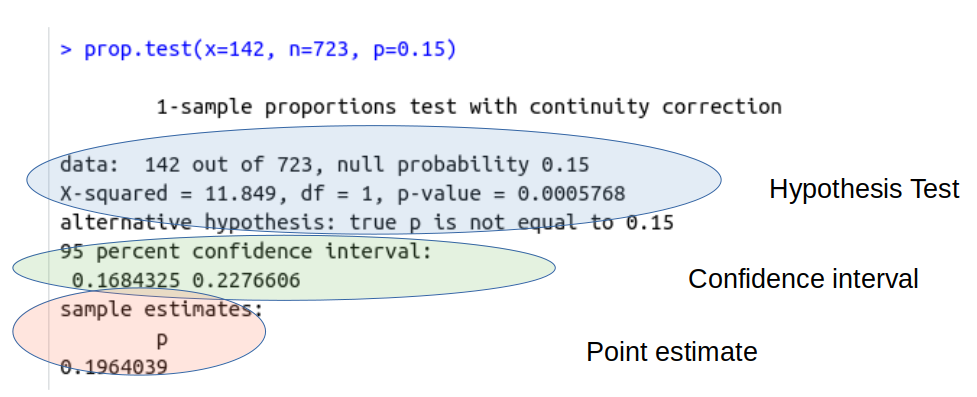
\includegraphics[width=1\linewidth]{images/propTestsAndCI} \end{figure}
\end{frame}

\begin{frame}[fragile]{Exercise 3}
\protect\hypertarget{exercise-3}{}
\begin{itemize}
\item
  In the diabetes dataset.

  \begin{itemize}
  \tightlist
  \item
    Test the hypothesis that the proportion of patients with
    \texttt{bmi30} is higher than 40\%

    \begin{itemize}
    \tightlist
    \item
      In the global population of the study
    \item
      Only in patients with `mort' equal ``Muerto''
    \end{itemize}
  \end{itemize}
\end{itemize}
\end{frame}

\begin{frame}{Contingency tables}
\protect\hypertarget{contingency-tables}{}
\begin{itemize}
\item
  A contingency table (a.k.a cross tabulation or cross tab) is a
  matrix-like table that displays the (multivariate) frequency
  distribution of the variables.
\item
  It is bidimensional, and classifies all observations according to two
  categorical variables (A and B, rows and columns).
\end{itemize}

\begin{figure}
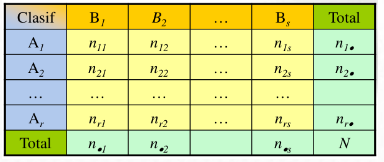
\includegraphics[width=0.8\linewidth]{images/contingencytables1} \end{figure}
\end{frame}

\begin{frame}{Chi-squared test}
\protect\hypertarget{chi-squared-test}{}
\begin{itemize}
\tightlist
\item
  A \emph{familiy} of tests receiving its name because they all rely on
  the \emph{Chi-Squared distribution} to compute the test probabilities.
\end{itemize}

\textbf{Chi squared independence test}

\begin{itemize}
\tightlist
\item
  When the sample comes from a single population with 2 categorical
  variables, the aim is to determine if there is relationship between
  them.
\end{itemize}

\textbf{Chi squared homogeneity test}

\begin{itemize}
\tightlist
\item
  When each row is a sample from distinct populations (groups,
  subgroups\ldots), the aim is to determine if both groups have
  significative differences in that variable
\end{itemize}
\end{frame}

\begin{frame}{Chi-squared tests}
\protect\hypertarget{chi-squared-tests}{}
\begin{itemize}
\item
  When we have:

  \begin{itemize}
  \tightlist
  \item
    quantitative data,
  \item
    two or more categories,
  \item
    independent observations,
  \item
    adequate sample size (\textgreater10)
  \end{itemize}
\item
  and our questions are like\ldots{}

  \begin{itemize}
  \item
    \emph{Do the number of individuals or objects that fall in each pair
    of categories differ significantly from the number you would expect
    if there was no association?}
  \item
    \emph{Is this difference between the expected and observed due to
    chance (``sampling variation''), or is it a real difference?}
  \end{itemize}
\end{itemize}
\end{frame}

\begin{frame}{Chi squared.test: Observed vs expected}
\protect\hypertarget{chi-squared.test-observed-vs-expected}{}
\begin{figure}
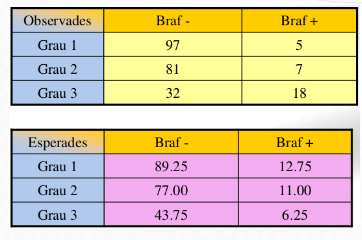
\includegraphics[width=0.8\linewidth]{images/observedvsexpected} \end{figure}
\end{frame}

\begin{frame}[fragile]{Chi squared tests: Observed vs expected with R}
\protect\hypertarget{chi-squared-tests-observed-vs-expected-with-r}{}
\begin{Shaded}
\begin{Highlighting}[]
\FunctionTok{require}\NormalTok{(gmodels)}
\NormalTok{mytable }\OtherTok{\textless{}{-}} \FunctionTok{table}\NormalTok{(dadescancer}\SpecialCharTok{$}\NormalTok{cancer, dadescancer}\SpecialCharTok{$}\NormalTok{fumar)}
\FunctionTok{CrossTable}\NormalTok{(mytable,}\AttributeTok{expected =}\NormalTok{ T,}\AttributeTok{prop.chisq =}\NormalTok{ F,}\AttributeTok{prop.c =}\NormalTok{ F,}\AttributeTok{prop.r =}\NormalTok{ F)}
\end{Highlighting}
\end{Shaded}

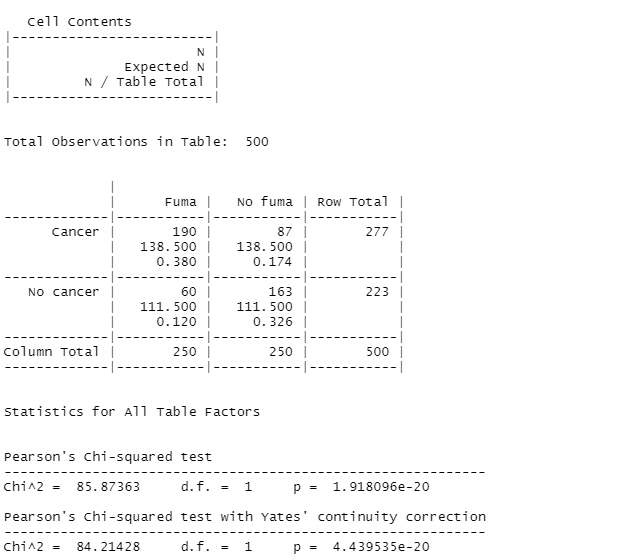
\includegraphics{images/chi.PNG}
\end{frame}

\begin{frame}[fragile]{Chi squared tests with R}
\protect\hypertarget{chi-squared-tests-with-r}{}
\begin{Shaded}
\begin{Highlighting}[]
\FunctionTok{chisq.test}\NormalTok{ (mytable)}
\end{Highlighting}
\end{Shaded}

\begin{verbatim}
## 
##  Pearson's Chi-squared test with Yates' continuity correction
## 
## data:  mytable
## X-squared = 84.214, df = 1, p-value < 2.2e-16
\end{verbatim}
\end{frame}

\begin{frame}[fragile]{Fisher test. an assumptions-free alternative}
\protect\hypertarget{fisher-test.-an-assumptions-free-alternative}{}
Chi-squared test require that sample sizes are ``big'' and expected
frequencies are, at least greater than 5.

Fisher test can be an alternative if these assumptions are not met,
especially for two times two tables.

\begin{Shaded}
\begin{Highlighting}[]
\FunctionTok{fisher.test}\NormalTok{(mytable)}
\end{Highlighting}
\end{Shaded}

\begin{verbatim}
## 
##  Fisher's Exact Test for Count Data
## 
## data:  mytable
## p-value < 2.2e-16
## alternative hypothesis: true odds ratio is not equal to 1
## 95 percent confidence interval:
##  3.945907 8.936465
## sample estimates:
## odds ratio 
##   5.909114
\end{verbatim}
\end{frame}

\begin{frame}[fragile]{Exercise 4}
\protect\hypertarget{exercise-4}{}
\begin{itemize}
\item
  Use the diabetes dataset to study if it can be detected an association
  between the variables \texttt{mort} and \texttt{tabac} in the diabetes
  dataset.
\item
  Do not start with a test but with an appropriate summarization and
  visualization!
\end{itemize}
\end{frame}

\begin{frame}{Mcnemar test}
\protect\hypertarget{mcnemar-test}{}
Mcnemar test is used to compare the frequencies of paired samples of
dichotomous data

\begin{itemize}
\item
  Ho: There is no significant change in individuals after the treatment
\item
  H1: There is a significant change in individuals after the treatment
\end{itemize}
\end{frame}

\begin{frame}[fragile]{Mcnemar test. Example}
\protect\hypertarget{mcnemar-test.-example}{}
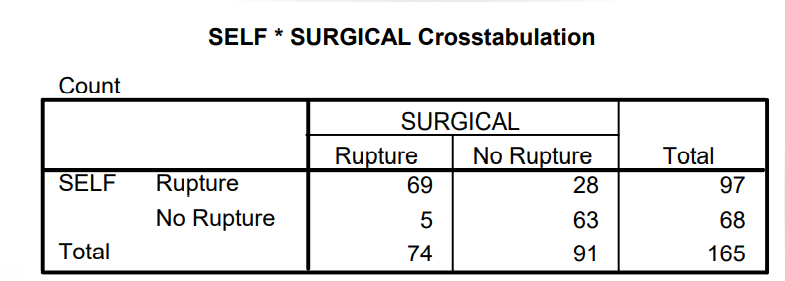
\includegraphics{images/mcnemar.PNG}

\begin{Shaded}
\begin{Highlighting}[]
\NormalTok{.Table }\OtherTok{\textless{}{-}} \FunctionTok{matrix}\NormalTok{(}\FunctionTok{c}\NormalTok{(}\DecValTok{69}\NormalTok{,}\DecValTok{28}\NormalTok{,}\DecValTok{5}\NormalTok{,}\DecValTok{63}\NormalTok{), }\DecValTok{2}\NormalTok{, }\DecValTok{2}\NormalTok{, }\AttributeTok{byrow=}\ConstantTok{TRUE}\NormalTok{)}
\FunctionTok{mcnemar.test}\NormalTok{(.Table)}
\end{Highlighting}
\end{Shaded}

\begin{verbatim}
## 
##  McNemar's Chi-squared test with continuity correction
## 
## data:  .Table
## McNemar's chi-squared = 14.667, df = 1, p-value = 0.0001283
\end{verbatim}
\end{frame}

\end{document}
